\section{Empirical study of executions disrupted by faults}\label{sec:empirical}
To visualize the impact of soft-errors on the convergence, different faults are injected into GMRES executions. First qualitative results on a few cases are given to illustrate in detail each fault parameter, and then, more quantitative experiments  using several matrices are performed to evaluate more extensively the fault effects. 

\subsection{Representation of executions}
Since an execution can be represented in many different ways, we propose in the following two visualizations enabling the key information to be displayed. The main purpose of the GMRES algorithm is to reduce the residual norm to the target accuracy, hence we use its convergence history, referring to the residual norm evolution through the iterations. Figure~\ref{fig:gre_216a_conv_hist} plots the convergence history of a GMRES execution on gre_216a, disrupted by a transient fault, as well as the same non-faulty execution for reference. We first observe that the true residual in the non-faulty execution (dashed blue curve) converges in $150$ iterations since it reaches the target accuracy ($\varepsilon = 10^{-12}$) at iteration 150. Then, the computed residual in the faulty execution also converges but much later (around iteration 195). On the contrary, the true residual in the faulty execution never reaches the target accuracy, as it remains greater than $10^{-7}$, so according to the definition, the faulty execution fails to converge. The fault (occurring at iteration 70) is responsible for this failure, and it can also be seen that after the fault occurrence, the residual norm decreases more slowly in the faulty execution, which imply more iterations than the reference and potentially a delayed solution (correct or incorrect).

The second way used to represent an execution is simply by its outcome. For instance, Table~\ref{table:outcomes} represent a set of outcomes used later in this section.






\begin{figure}[h]
		\centering
		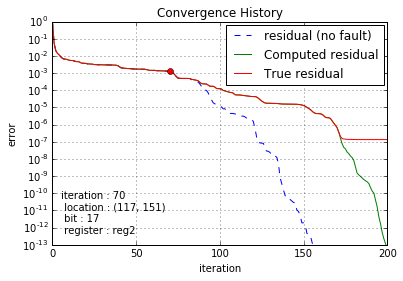
\includegraphics[width=0.8\linewidth]{figures/gre_216a/convergence_history_fault.png}	
	\caption{Convergence history of a GMRES execution on gre_216a disrupted by a transient fault (red circle). The Y axis corresponds to the residual norm, and the X axis is the iteration where it was measured. The dashed blue line corresponds to the true residual norm in the reference non-faulty execution, the red line is the true residual norm in the faulty execution (the fault parameters are displayed at the bottom left hand corner) and the green line is the computed residual norm in the faulty execution.}\label{fig:gre_216a_conv_hist}
\end{figure}



\begin{table}[h]
\centering
\caption{Color used for each test outcome.}
\label{table:outcomes}
\begin{tabular}{|c|}
\hline
	Outcome  \tabularnewline
    \hline
 \color[RGB]{50, 150, 50}{\textbf{Convergence without delay}} \\
 \color{blue}{\textbf{Convergence with delay}} \\
 \color{red}{\textbf{No convergence}} \\

    \hline
\end{tabular}
\end{table}



\subsection{Qualitative results and parameters influence}
To visualize the influence of each fault parameter, the convergence history of 3 disrupted GMRES executions over the same matrices (HB/gre_216a for GMRES and HB/pores_2 for preconditioned-GMRES) are plotted for each 4 parameters (bit flipped, iteration, register and location). 

In Figure \ref{fig:conv_hist_bit} all parameters but the bit flipped are fixed. It can be observed that bit-flips on the most significant bits have a stronger impact on the convergence than bit-flips on the least significant bits: in Figure~\ref{fig:gre_216a_conv_hist_bit_0}, the bit flipped is one of the register's least significant bit (bit 60) and the fault does not prevent the convergence. In Figure~\ref{fig:gre_216a_conv_hist_bit_1}, the $40^{th}$ bit is flipped and the convergence is delayed by a dozen iterations. In Figure \ref{fig:gre_216a_conv_hist_bit_2} the $20^{th}$ bit is flipped and the execution never converges to the target accuracy.
Intuitively, bit flips on the most significant bits introduce bigger errors and are more likely to disrupt the convergence than bit flips on the least significant bits.





\begin{figure}[h]
	\centering
    
\begin{minipage}[b]{0.45\linewidth}
\centering
\textbf{GMRES} executions on \textbf{gre_216a} 
\end{minipage}
\quad
\begin{minipage}{0.45\linewidth}
\centering
\textbf{preconditioned-GMRES} on \textbf{pores_2}
\end{minipage}\\


    \begin{minipage}[b]{0.48\linewidth}
	\begin{subfigure}[t]{\linewidth}
		\centering
		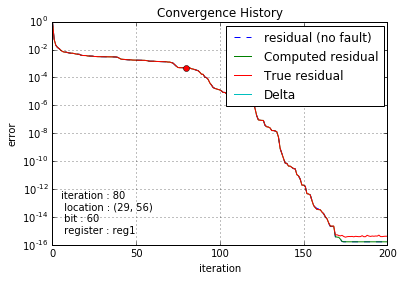
\includegraphics[width=\linewidth]{figures/gre_216a/convergence_history_bit_0.png}
		\caption{bit 60}\label{fig:gre_216a_conv_hist_bit_0}		
	\end{subfigure}
	\quad
	\begin{subfigure}[t]{\linewidth}
		\centering
		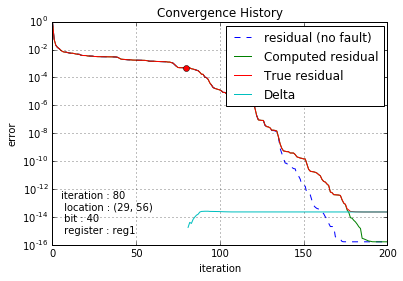
\includegraphics[width=\linewidth]{figures/gre_216a/convergence_history_bit_1.png}
		\caption{bit 40}\label{fig:gre_216a_conv_hist_bit_1}
	\end{subfigure}
    \quad
    \begin{subfigure}[t]{\linewidth}
		\centering
		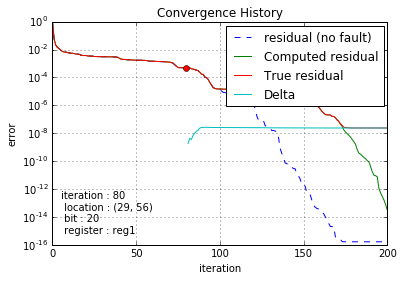
\includegraphics[width=\linewidth]{figures/gre_216a/convergence_history_bit_2.png}
		\caption{bit 20}\label{fig:gre_216a_conv_hist_bit_2}
	\end{subfigure}
    \end{minipage}
    \quad
    \begin{minipage}[b]{0.48\linewidth}
    	\begin{subfigure}[t]{\linewidth}
		\centering
		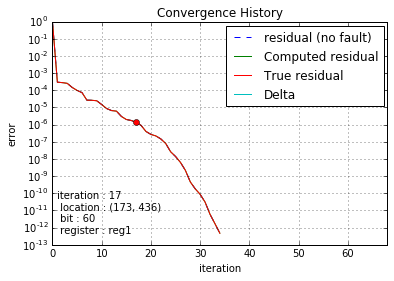
\includegraphics[width=\linewidth]{figures/pores_2/convergence_history_bit_0.png}
		\caption{bit 60}\label{fig:pores_2_conv_hist_bit_0}		
	\end{subfigure}
	\quad
	\begin{subfigure}[t]{\linewidth}
		\centering
		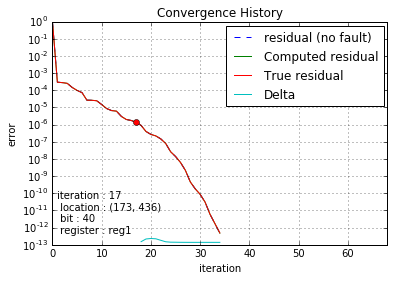
\includegraphics[width=\linewidth]{figures/pores_2/convergence_history_bit_1.png}
		\caption{bit 40}\label{fig:pores_2_conv_hist_bit_1}
	\end{subfigure}
    \quad
    \begin{subfigure}[t]{\linewidth}
		\centering
		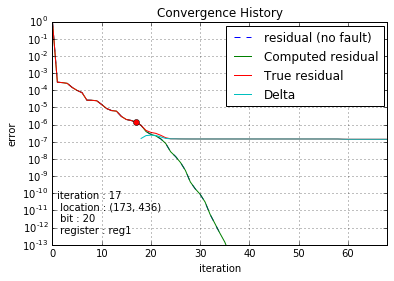
\includegraphics[width=\linewidth]{figures/pores_2/convergence_history_bit_2.png}
		\caption{bit 20}\label{fig:pores_2_conv_hist_bit_2}
	\end{subfigure}

    
	\end{minipage}
\caption{Convergence history of 3 GMRES executions on gre_216a and 3 preconditioned-GMRES executions on pores_2, disrupted by a transient fault. In the execution \ref{fig:gre_216a_conv_hist_bit_0}, the fault (\textbf{bit 20}) disrupts the convergence, in \ref{fig:gre_216a_conv_hist_bit_1}, the fault (\textbf{bit 40}) delays it, and in \ref{fig:gre_216a_conv_hist_bit_2}, the fault (\textbf{bit 60}) has no effect on the convergence.}\label{fig:conv_hist_bit}
\end{figure}



In Figure~\ref{fig:conv_hist_iteration}, all parameters but the iteration when the fault occurs are fixed. It can be observed in both GMRES and preconditioned-GMRES that the sooner the fault occurred, the bigger the impact on convergence seems to be: in Figure \ref{fig:gre_216a_conv_hist_iteration_0}, the fault occurred on the $1^{st}$ iteration and the execution did not converge, in Figure \ref{fig:gre_216a_conv_hist_iteration_1}, the fault occurs on the $61^{st}$ iteration and the convergence is delayed, and in Figure \ref{fig:gre_216a_conv_hist_iteration_2} the fault occurs on the $121^{st}$ iteration and the execution converges to the target accuracy.
This observations complies with the intuition that the first iterations are responsible for the main part of the solution, while latter ones are responsible for its refinement, hence faults are more likely to be critical when occurring at the early stages of the execution than towards the end.





\begin{figure}[h]
	\centering
    
\begin{minipage}[b]{0.45\linewidth}
\centering
\textbf{GMRES} executions on \textbf{gre_216a} 
\end{minipage}
\quad
\begin{minipage}{0.45\linewidth}
\centering
\textbf{preconditioned-GMRES} on \textbf{pores_2}
\end{minipage}\\


    \begin{minipage}[b]{0.48\linewidth}
	\begin{subfigure}[t]{\linewidth}
		\centering
		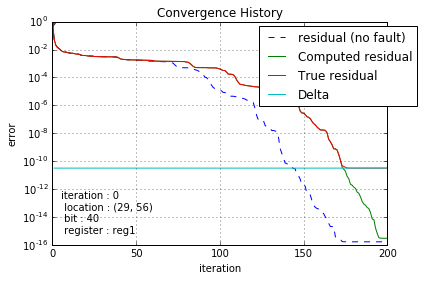
\includegraphics[width=\linewidth]{figures/gre_216a/convergence_history_iteration_0.png}
		\caption{iteration 0}\label{fig:gre_216a_conv_hist_iteration_0}		
	\end{subfigure}
	\quad
	\begin{subfigure}[t]{\linewidth}
		\centering
		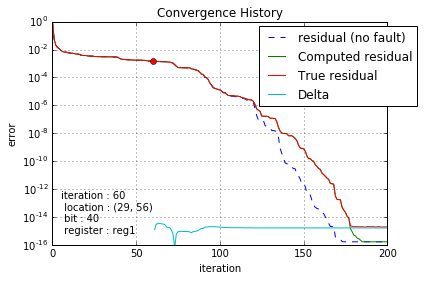
\includegraphics[width=\linewidth]{figures/gre_216a/convergence_history_iteration_1.png}
		\caption{iteration 60}\label{fig:gre_216a_conv_hist_iteration_1}
	\end{subfigure}
    \quad
    \begin{subfigure}[t]{\linewidth}
		\centering
		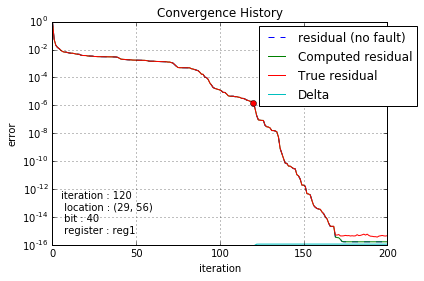
\includegraphics[width=\linewidth]{figures/gre_216a/convergence_history_iteration_2.png}
		\caption{iteration 120}\label{fig:gre_216a_conv_hist_iteration_2}
	\end{subfigure}
    \end{minipage}
    \quad
    \begin{minipage}[b]{0.48\linewidth}
    	\begin{subfigure}[t]{\linewidth}
		\centering
		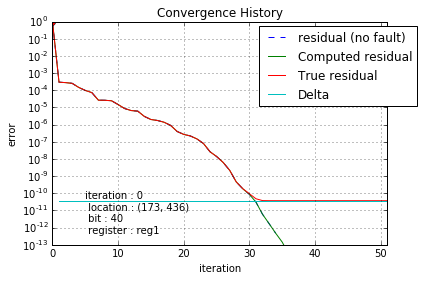
\includegraphics[width=\linewidth]{figures/pores_2/convergence_history_iteration_0.png}
		\caption{iteration 0}\label{fig:pores_2_conv_hist_iteration_0}		
	\end{subfigure}
	\quad
	\begin{subfigure}[t]{\linewidth}
		\centering
		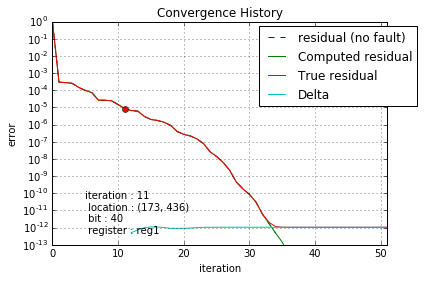
\includegraphics[width=\linewidth]{figures/pores_2/convergence_history_iteration_1.png}
		\caption{iteration 11}\label{fig:pores_2_conv_hist_iteration_1}
	\end{subfigure}
    \quad
    \begin{subfigure}[t]{\linewidth}
		\centering
		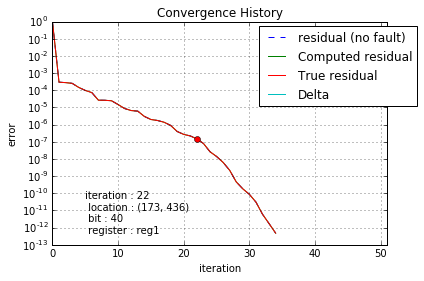
\includegraphics[width=\linewidth]{figures/pores_2/convergence_history_iteration_2.png}
		\caption{iteration 22}\label{fig:pores_2_conv_hist_iteration_2}
	\end{subfigure}

    
	\end{minipage}
\caption{Convergence history of 3 GMRES executions on gre_216a and 3 preconditioned-GMRES executions on pores_2, disrupted by a transient fault. In the execution \ref{fig:gre_216a_conv_hist_iteration_0}, the fault (\textbf{iteration 0}) disrupts the convergence, in \ref{fig:gre_216a_conv_hist_iteration_1}, the fault (\textbf{iteration 60}) delays it, and in \ref{fig:gre_216a_conv_hist_iteration_2}, the fault (\textbf{iteration 120}) has no effect on the convergence.}\label{fig:conv_hist_iteration}
\end{figure}




The remaining fault parameters (register and location) do not appear to have any significant impact on the convergence, even though inputs can be constructed to contradict this observation. Figure \ref{fig:conv_hist_register}, representing the convergence history of 3 GMRES executions and 3 preconditioned-GMRES disrupted by a bit-flip on $reg_1$, $reg_2$ and $reg_3$, and Figure \ref{fig:conv_hist_location}, representing the convergence history of 3 GMRES executions and 3 preconditioned-GMRES disrupted by a bit-flip on three different locations, present similar behaviors in terms of convergence history.



\begin{figure}[h]
	\centering
    
\begin{minipage}[b]{0.45\linewidth}
\centering
\textbf{GMRES} executions on \textbf{gre_216a} 
\end{minipage}
\quad
\begin{minipage}{0.45\linewidth}
\centering
\textbf{preconditioned-GMRES} on \textbf{pores_2}
\end{minipage}\\


    \begin{minipage}[b]{0.48\linewidth}
	\begin{subfigure}[t]{\linewidth}
		\centering
		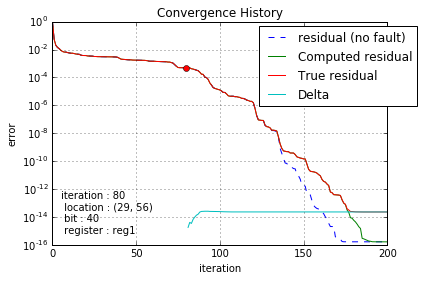
\includegraphics[width=\linewidth]{figures/gre_216a/convergence_history_register_0.png}
		\caption{$reg_1$}\label{fig:gre_216a_conv_hist_register_0}		
	\end{subfigure}
	\quad
	\begin{subfigure}[t]{\linewidth}
		\centering
		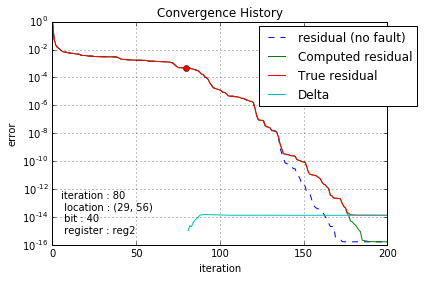
\includegraphics[width=\linewidth]{figures/gre_216a/convergence_history_register_1.png}
		\caption{$reg_2$}\label{fig:gre_216a_conv_hist_register_1}
	\end{subfigure}
    \quad
    \begin{subfigure}[t]{\linewidth}
		\centering
		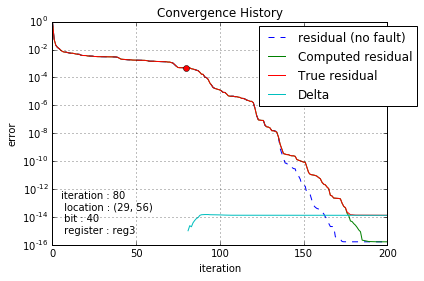
\includegraphics[width=\linewidth]{figures/gre_216a/convergence_history_register_2.png}
		\caption{$reg_3$}\label{fig:gre_216a_conv_hist_register_2}
	\end{subfigure}
    \end{minipage}
    \quad
    \begin{minipage}[b]{0.48\linewidth}
    	\begin{subfigure}[t]{\linewidth}
		\centering
		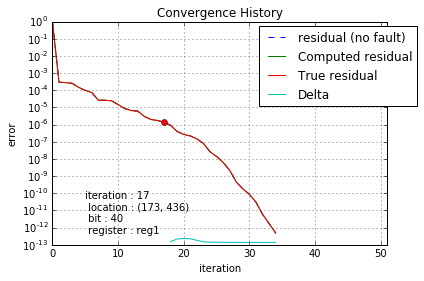
\includegraphics[width=\linewidth]{figures/pores_2/convergence_history_register_0.png}
		\caption{$reg_1$}\label{fig:pores_2_conv_hist_register_0}		
	\end{subfigure}
	\quad
	\begin{subfigure}[t]{\linewidth}
		\centering
		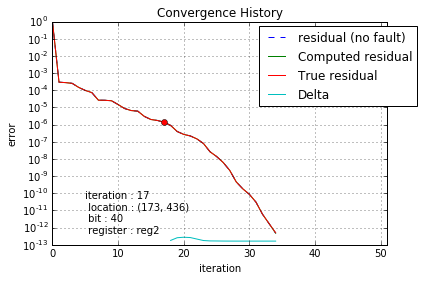
\includegraphics[width=\linewidth]{figures/pores_2/convergence_history_register_1.png}
		\caption{$reg_2$}\label{fig:pores_2_conv_hist_register_1}
	\end{subfigure}
    \quad
    \begin{subfigure}[t]{\linewidth}
		\centering
		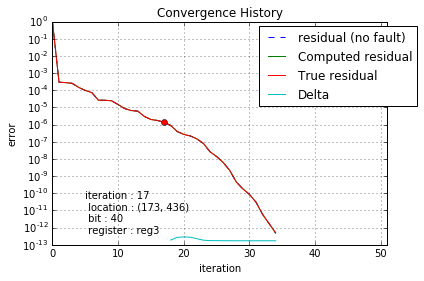
\includegraphics[width=\linewidth]{figures/pores_2/convergence_history_register_2.png}
		\caption{$reg_3$}\label{fig:pores_2_conv_hist_register_2}
	\end{subfigure}

    
	\end{minipage}
	\caption{Convergence history of 3 GMRES executions on gre_216a and 3 preconditioned-GMRES executions on pores_2, disrupted by a transient fault. In all the executions, the faults (occurring in $reg_1$, $reg_2$ and $reg_3$) seem to have the same impact.}\label{fig:conv_hist_register}
\end{figure}







\begin{figure}[h]
	\centering
    
\begin{minipage}[b]{0.45\linewidth}
\centering
\textbf{GMRES} executions on \textbf{gre_216a} 
\end{minipage}
\quad
\begin{minipage}{0.45\linewidth}
\centering
\textbf{preconditioned-GMRES} on \textbf{pores_2}
\end{minipage}\\


    \begin{minipage}[b]{0.48\linewidth}
	\begin{subfigure}[t]{\linewidth}
		\centering
		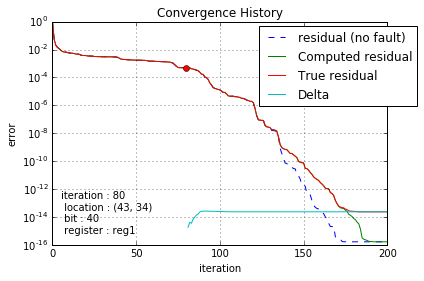
\includegraphics[width=\linewidth]{figures/gre_216a/convergence_history_location_0.png}
		\caption{}\label{fig:gre_216a_conv_hist_location_0}		
	\end{subfigure}
	\quad
	\begin{subfigure}[t]{\linewidth}
		\centering
		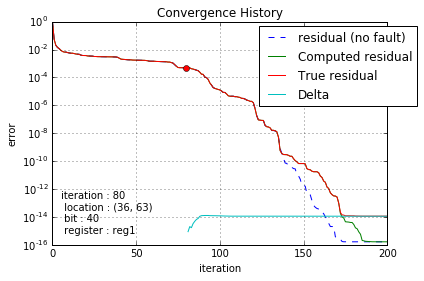
\includegraphics[width=\linewidth]{figures/gre_216a/convergence_history_location_1.png}
		\caption{}\label{fig:gre_216a_conv_hist_location_1}
	\end{subfigure}
    \quad
    \begin{subfigure}[t]{\linewidth}
		\centering
		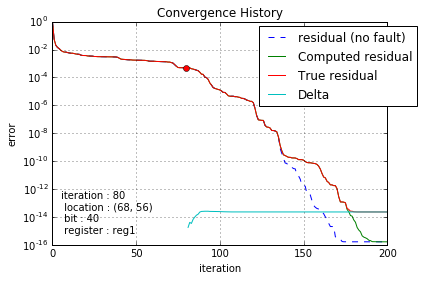
\includegraphics[width=\linewidth]{figures/gre_216a/convergence_history_location_2.png}
		\caption{}\label{fig:gre_216a_conv_hist_location_2}
	\end{subfigure}
    \end{minipage}
    \quad
    \begin{minipage}[b]{0.48\linewidth}
    	\begin{subfigure}[t]{\linewidth}
		\centering
		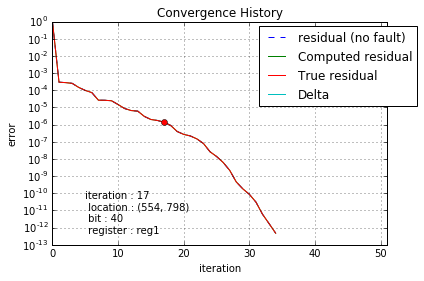
\includegraphics[width=\linewidth]{figures/pores_2/convergence_history_location_0.png}
		\caption{}\label{fig:pores_2_conv_hist_location_0}		
	\end{subfigure}
	\quad
	\begin{subfigure}[t]{\linewidth}
		\centering
		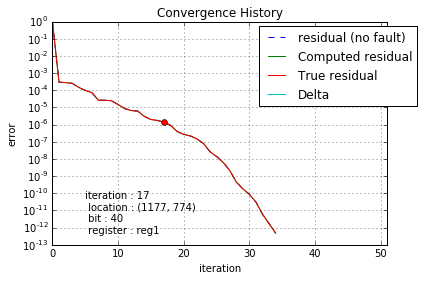
\includegraphics[width=\linewidth]{figures/pores_2/convergence_history_location_1.png}
		\caption{}\label{fig:pores_2_conv_hist_location_1}
	\end{subfigure}
    \quad
    \begin{subfigure}[t]{\linewidth}
		\centering
		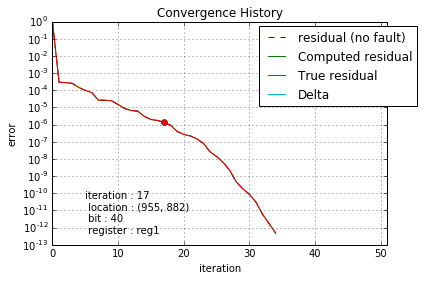
\includegraphics[width=\linewidth]{figures/pores_2/convergence_history_location_2.png}
		\caption{}\label{fig:pores_2_conv_hist_location_2}
	\end{subfigure}

    
	\end{minipage}
	\caption{Convergence history of 3 GMRES executions on gre_216a and 3 preconditioned-GMRES executions on pores_2, disrupted by a transient fault. In all the executions, the faults (occurring in random locations) seem to have the same impact.}\label{fig:conv_hist_location}
\end{figure}


\subsection{Quantitative results}

To illustrate the previous observation, Figure~\ref{fig:bit_iteration} presents the convergence of several faulty-executions - one for each couple (iteration fault $\times$ bit flipped) while the other parameters are chosen randomly - for GMRES on HB/gre_216a and preconditioned-GMRES on HB/pores_2. Some faults have no effect on the convergence (in green), some may only delay it (blue), and others may prevent the execution from converging to the target accuracy (red). As observed in the previous results, faults involving the most significant bits of the registers or happening soon in the execution are more likely to cause a failure than faults involving the least significant bits or happening late in the execution.






\begin{figure}[ht] 
\hspace{3ex}
\begin{minipage}[b]{0.5\linewidth}
\centering
\textbf{GMRES} executions on \textbf{gre_216a} 
\end{minipage}
\quad
\begin{minipage}{0.5\linewidth}
\centering
\textbf{preconditioned-GMRES} on \textbf{pores_2}
\end{minipage}\\

  \begin{subfigure}[b]{0.5\linewidth}
    \centering
	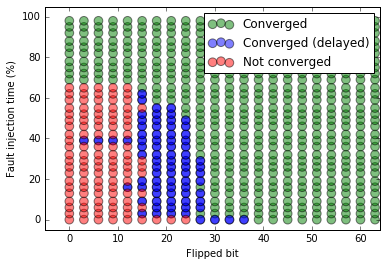
\includegraphics[width=\linewidth]{figures/gre_216a/bit_iteration_0.png} %TODO
	\caption{$\varepsilon = 10^{-6}$}
    \label{fig:gre_216a_bit_iteration_0}	
  \end{subfigure}%% 
   \hspace{4ex}
  \begin{subfigure}[b]{0.5\linewidth}
    \centering
    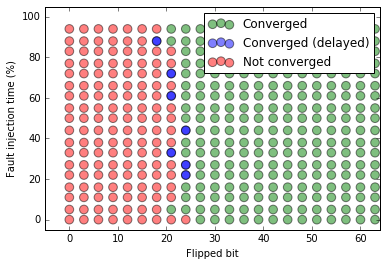
\includegraphics[width=\linewidth]{figures/pores_2/bit_iteration_0.png} %TODO
	\caption{$\varepsilon = 10^{-6}$}
    \label{fig:pores_2_bit_iteration_0}	
  \end{subfigure} 

  \begin{subfigure}[b]{0.5\linewidth}
    \centering
 	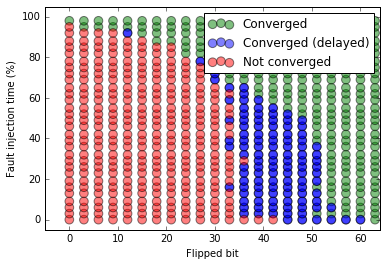
\includegraphics[width=\linewidth]{figures/gre_216a/bit_iteration_1.png} %TODO
	\caption{$\varepsilon = 10^{-12}$}
    \label{fig:gre_216a_bit_iteration_1}	
  \end{subfigure}%%
    \hspace{4ex}
  \begin{subfigure}[b]{0.5\linewidth}
    \centering
	 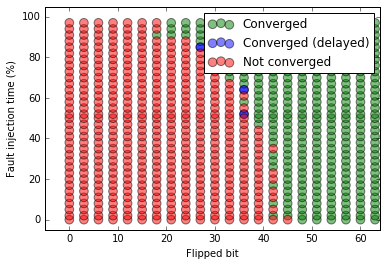
\includegraphics[width=\linewidth]{figures/pores_2/bit_iteration_1.png} %TODO
	\caption{$\varepsilon = 10^{-12}$}
    \label{fig:pores_2_bit_iteration_1}	
  \end{subfigure} 
\caption{Diagram of executions disrupted by a fault. Each dot represents an execution of GMRES on HB/gre_216a (figures \ref{fig:gre_216a_bit_iteration_0} and \ref{fig:gre_216a_bit_iteration_1}) or preconditioned-GMRES on HB/pores_2 (figures \ref{fig:pores_2_bit_iteration_0} and \ref{fig:pores_2_bit_iteration_1}), its abscissa is the bit where the fault occurred, its ordinate is the moment in the execution when the fault has been injected and its color represents whether the execution has converged or not (green: no delay, red: no convergence, blue: delayed convergence).}
\label{fig:bit_iteration}
\end{figure}





As shown in Figure~\ref{fig:matrices_bit_iteration}, the behavior of faulty GMRES is very similar for all the selected matrices: the left-hand side of the graphs corresponding to executions disrupted by bit-flips of the most significant bit mostly fail to converge, except for the latest iterations, while the right-hand side of the graphs corresponding to executions where the least significant bits are flipped usually converges. %TODO: refaire les graphs (légende + preconditioned-gmres)




\begin{figure}[ht] 
\hspace{3ex}


  \begin{subfigure}[b]{0.5\linewidth}
    \centering
	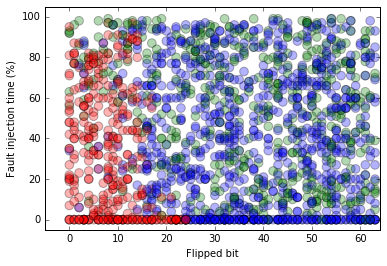
\includegraphics[width=\linewidth]{figures/bit_iteration_0.png} %TODO
	\caption{$\varepsilon = 10^{-6}$}
    \label{fig:bit_iteration_0}	
  \end{subfigure}%% 
   \hspace{4ex}
  \begin{subfigure}[b]{0.5\linewidth}
    \centering
    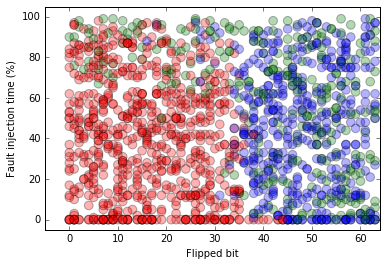
\includegraphics[width=\linewidth]{figures/bit_iteration_1.png} %TODO
	\caption{$\varepsilon = 10^{-12}$}
    \label{fig:bit_iteration_1}	
  \end{subfigure} 

\caption{Diagrams of GMRES executions disrupted by a fault. Each dot represents an execution on any matrix of the dataset, its abscissa is the bit where the fault occurred, its ordinate is the moment in the execution when the fault has been injected and its color represents whether the execution has converged or not (green: no delay, red: no convergence, blue: delayed convergence).}
\label{fig:matrices_bit_iteration}
\end{figure}








\newpage

%From \cite{DBLP:journals/siamsc/GiraudGL07} : 
%\begin{equation}\label{eqn:delta}
%	\text{delta = } \|\widetilde{r_l} - \widetilde{r_l}\textprime \| = ||y_{l, k}(z_{k+1} - z_{k+1})\| 
%\end{equation}
 
